% \input{"IAB/latex/TeX-Folienformat.tex"}
\input{"/Users/jonathanlatner/Google Drive/My Drive/IAB/latex/TeX-Folienformat.tex"}

\documentclass[t,8pt,utfx8]{beamer}
\usepackage{booktabs}
\usepackage{setspace}
\usepackage{parskip}
\usepackage{graphicx}
\usepackage{subcaption}
\setbeamertemplate{caption}[numbered]
\newcommand{\sprache}{\englisch}
\renewcommand{\thesubsection}{\alph{subsection})}
\usepackage[cal=pxtx, scr=dutchcal]{mathalpha}



\definecolor{codegreen}{rgb}{0,0.6,0}
\definecolor{codegray}{rgb}{0.5,0.5,0.5}
\definecolor{codepurple}{rgb}{0.58,0,0.82}
\definecolor{backcolour}{rgb}{0.95,0.95,0.92}



\newcommand{\btVFill}{\vskip0pt plus 1filll}


\title{Understanding the trade-off between utility and risk in CART based models using simulation data}
\subtitle{Berlin, \newline 7-8. Oktober, 2024}

\author{Jonathan Latner, PhD \newline Dr. Marcel Neuenhoeffer \newline Prof. Dr. Jörg Drechsler}

\newcounter{noauthorlines}
\setcounter{noauthorlines}{2} % Wert für 2 Autoren über 2 Zeilen. Ggf. anpassen

% %%%%%%%%%%%%%%
% Ende Anpassung
% %%%%%%%%%%%%%%

% \input{"IAB/latex/TeX-Folienformatierung_CD_2019"}
\input{"/Users/jonathanlatner/Google Drive/My Drive/IAB/latex/TeX-Folienformatierung_CD_2019"}

% Modify the section in toc template to enumerate
\setbeamertemplate{section in toc}{%
    \inserttocsectionnumber.~\inserttocsection\par
}

% use for subsections
% \setbeamertemplate{subsection in toc}{}
\setbeamertemplate{subsection in toc}{%
    \setlength{\parskip}{1mm}
        \hskip2mm -- \hskip1mm\inserttocsubsection\par
}


\usepackage{colortbl}
\definecolor{lightgray}{gray}{0.9}

\usepackage{listings} %include R code
\lstdefinestyle{mystyle}{
    backgroundcolor=\color{backcolour},   
    commentstyle=\color{codegreen},
    keywordstyle=\color{magenta},
    numberstyle=\tiny\color{codegray},
    stringstyle=\color{codepurple},
    basicstyle=\ttfamily\tiny,
    breakatwhitespace=false,         
    breaklines=true,                 
    captionpos=b,                    
    keepspaces=true,                 
    numbers=left,                    
    numbersep=5pt,                  
    showspaces=false,                
    showstringspaces=false,
    showtabs=false,                 
    columns=fullflexible,
    frame=single,
    tabsize=2
}
\lstset{style=mystyle}


\begin{document}


\frame[plain]{\titlepage}

\begin{spacing}{1.25}


%%%%%%%%%%%%%%%%%%%%%%%%%%%%%%%%%%%%%%%%
%%%%%%%%%%%%%%%%%%%%%%%%%%%%%%%%%%%%%%%%
\section{Introduction}\label{sec:intro}
%%%%%%%%%%%%%%%%%%%%%%%%%%%%%%%%%%%%%%%%
%%%%%%%%%%%%%%%%%%%%%%%%%%%%%%%%%%%%%%%%
\begin{frame}[c,plain]
\vskip-4mm
\begin{beamercolorbox}[wd=\boxwidth,ht=22.11mm]{transparent}%
    \vfill%
    \usebeamerfont{title}%
    \leftinsert%
    \MakeUppercase{Section \ref{sec:intro}: Introduction
} % <- Hier die Überschrift eintragen
\end{beamercolorbox}
\vskip-3mm
\pgfuseimage{rahmenlinie}
\end{frame}


\frame{\frametitle{Overview}

\begin{itemize}
    \item It is well established that there is a trade-off between utility and privacy when generating synthetic data
    \item We know the utility of CART models is really high
    \item Is it actually preserving privacy?
    \item Some measures indicate the answer is yes
    \item Wait a minute?  How does it preserve privacy and utility?
    \item Its hard to understand what exactly is happening
    \item Use toy data
    \item suggests its leaking information in non-obvious ways
    \item traditional post-hoc measures don't capture that
    \item Utility is really good, but its leaking information
    \item Here's how we convince you
    \item Traditional measures don't capture that, so we have to be careful
\end{itemize}
}

show an example of the trade-off

%%%%%%%%%%%%%%%%%%%%%%%%%%%%%%%%%%%%%%%%
%%%%%%%%%%%%%%%%%%%%%%%%%%%%%%%%%%%%%%%%
\section{Simulated data}\label{sec:data}
%%%%%%%%%%%%%%%%%%%%%%%%%%%%%%%%%%%%%%%%
%%%%%%%%%%%%%%%%%%%%%%%%%%%%%%%%%%%%%%%%
\frame{\frametitle{Data}
From Reiter et al., 2014

``We use a simple simulation scenario that illustrates many of the main issues: protecting a $2^4$ binary table with fully synthetic data. For $i = 1, \dots, 1000 = n$, let $y_i = (y_{1i}, y_{2i}, y_{3i}, y_{4i})$ comprise four binary variables. Let each of the $K = 16$ possible combinations be denoted $c_k$, where $k = 1,\dots,16$.  Let $c_{16} = (0,0,0,0)$, and let $C_{-16} = (c_1,\dots,c_{15})$. We generate an observed dataset $D$ as follows.  For $i = 1,...,n-1 = 999$, sample $y_i$ from a multinomial distribution such that $p(y_i = c_k) = 1/15$ for all $c_k \in C-16$. Set $y_{1000} = c_{16}$. Since we do full synthesis, $X = \theta$''
}


\frame{\frametitle{Variable frequency}
\begin{figure}
    \caption{}
    \resizebox{\textwidth}{!}{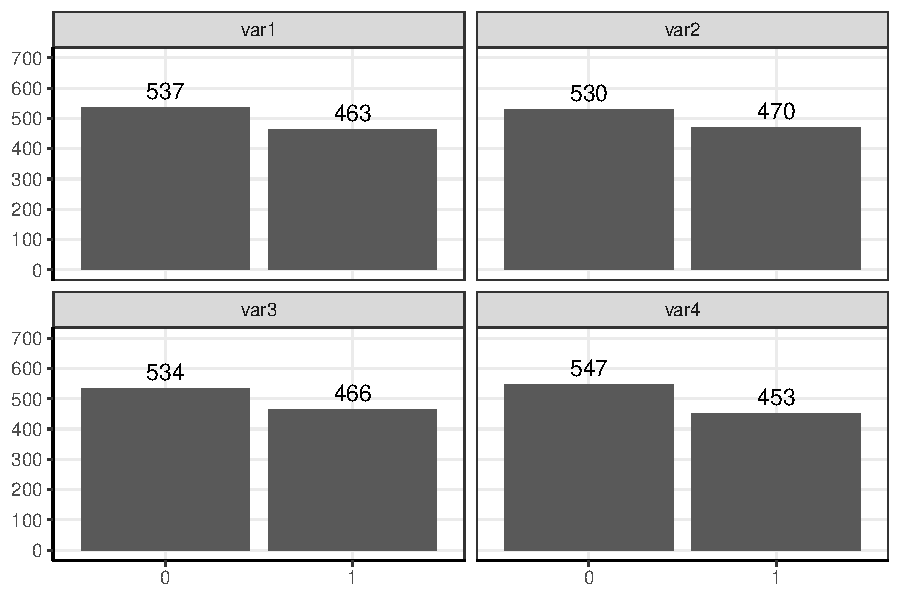
\includegraphics{../../graphs/graph_numeric_frequency.pdf}}
    \label{fig:graph_numeric_frequency}
\end{figure}
}

\frame{\frametitle{Histogram}
\begin{figure}
    \caption{}
    \resizebox{\textwidth}{!}{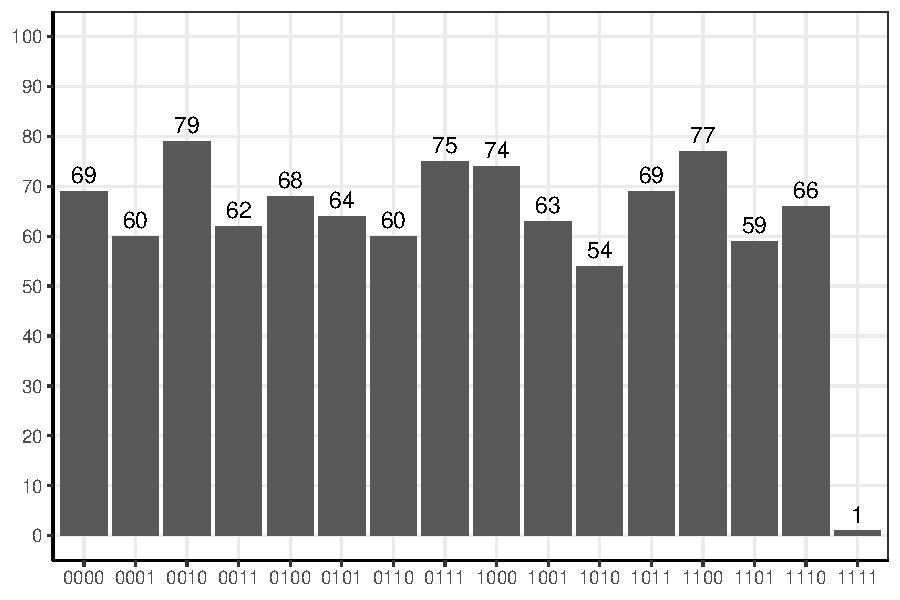
\includegraphics{../../graphs/graph_numeric_histogram.pdf}}
    \label{fig:graph_numeric_histogram}
\end{figure}
}

\begin{frame}[fragile]
\frametitle{Synthpop}

\begin{lstlisting}
> sds <- syn(df_ods, m=1)
Warning: In your synthesis there are numeric variables with 5 or fewer levels: var1, var2, var3, var4.
Consider changing them to factors. You can do it using parameter 'minnumlevels'.

Synthesis
-----------
 var1 var2 var3 var4
\end{lstlisting}

notice the "Warning".  It means that the variables are being synthesized as numerical values  (0/1), and Synthpop is suggesting they should be synthesized as categorical values  (``0''/``1'')
\end{frame}

\frame{\frametitle{Compare frequency (numerical)}
\begin{figure}
    \caption{}
    \resizebox{\textwidth}{!}{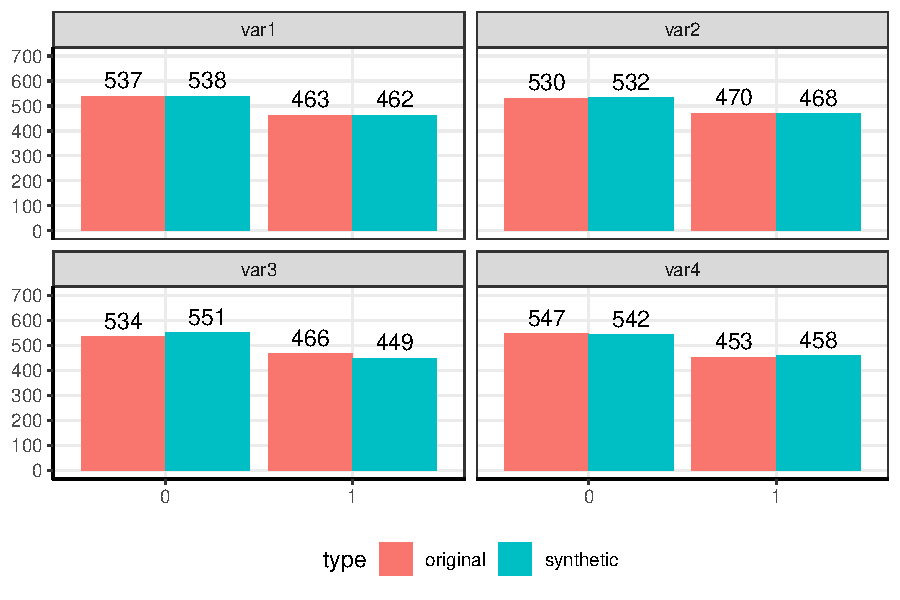
\includegraphics{../../graphs/graph_numeric_compare_frequency.pdf}}
    \label{fig:graph_numeric_compare_frequency}
\end{figure}
}

\frame{\frametitle{Compare histogram (numerical)}
\begin{figure}
    \caption{}
    \resizebox{\textwidth}{!}{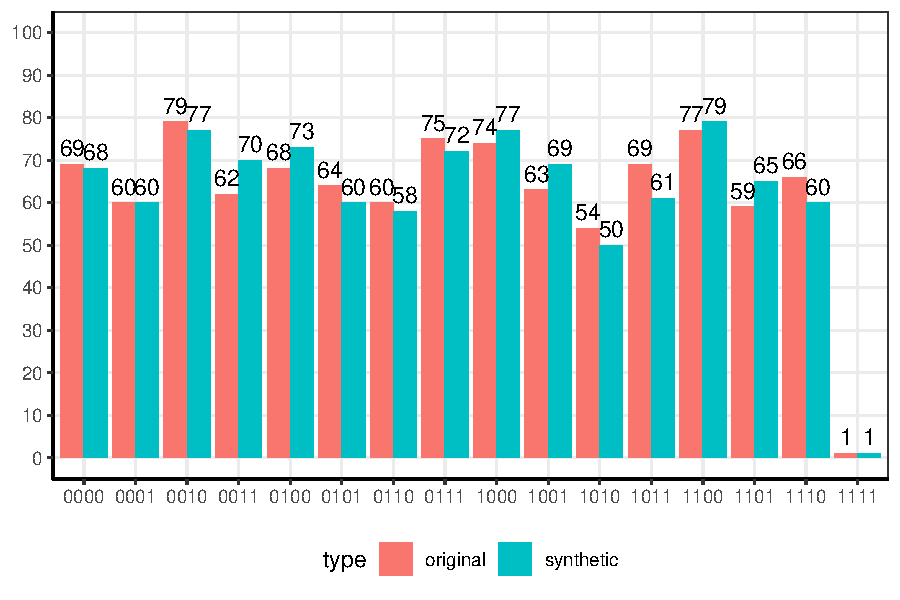
\includegraphics{../../graphs/graph_numeric_compare_histogram.pdf}}
    \label{fig:graph_numeric_compare_histogram}
\end{figure}
}

\frame{\frametitle{Compare histogram (numerical) x 100 synthetic datasets}
\begin{figure}
    \caption{}
    \resizebox{\textwidth}{!}{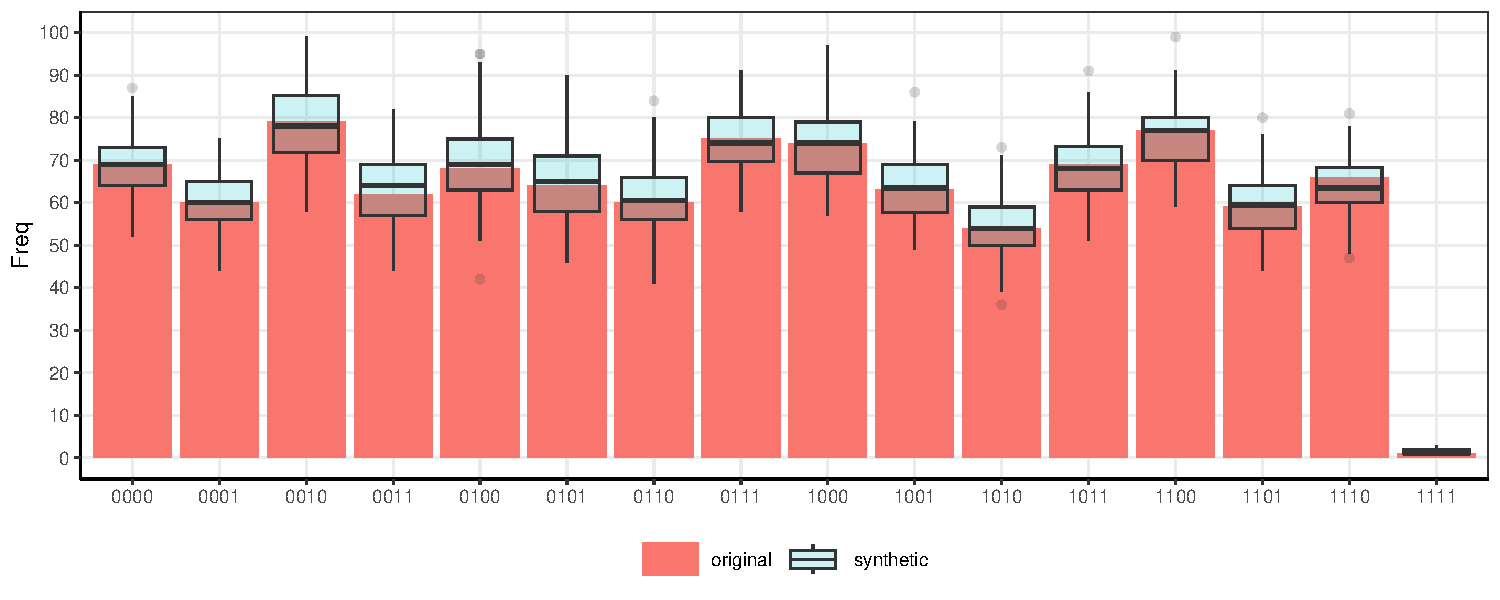
\includegraphics{../../graphs/graph_numeric_compare_histogram_100.pdf}}
    \label{fig:graph_numeric_compare_histogram_100}
\end{figure}
}

\frame{\frametitle{Compare frequency (categorical)}
\begin{figure}
    \caption{}
    \resizebox{\textwidth}{!}{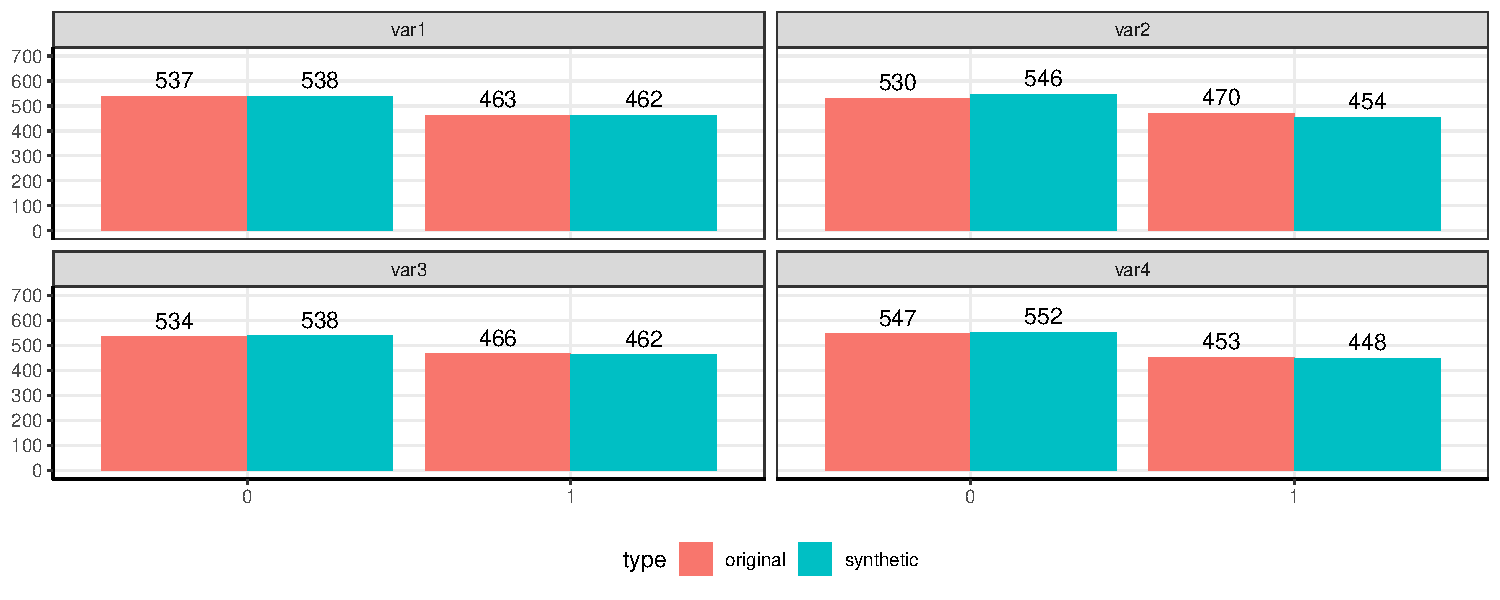
\includegraphics{../../graphs/graph_categorical_compare_frequency.pdf}}
    \label{fig:graph_categorical_compare_frequency}
\end{figure}
}

\frame{\frametitle{Compare histogram (categorical)}
\begin{figure}
    \caption{}
    \resizebox{\textwidth}{!}{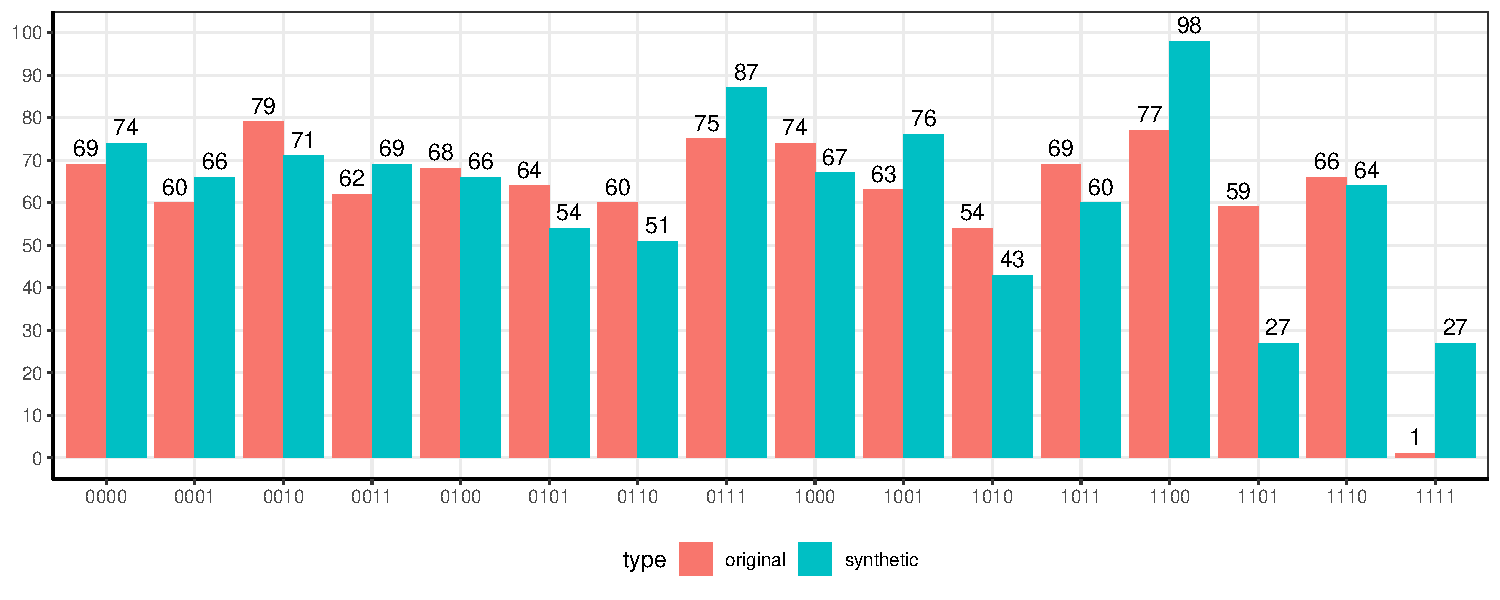
\includegraphics{../../graphs/graph_categorical_compare_histogram.pdf}}
    \label{fig:graph_categorical_compare_histogram}
\end{figure}
}

\frame{\frametitle{Compare histogram (categorical) x 100 synthetic datasets}
\begin{figure}
    \caption{}
    \resizebox{\textwidth}{!}{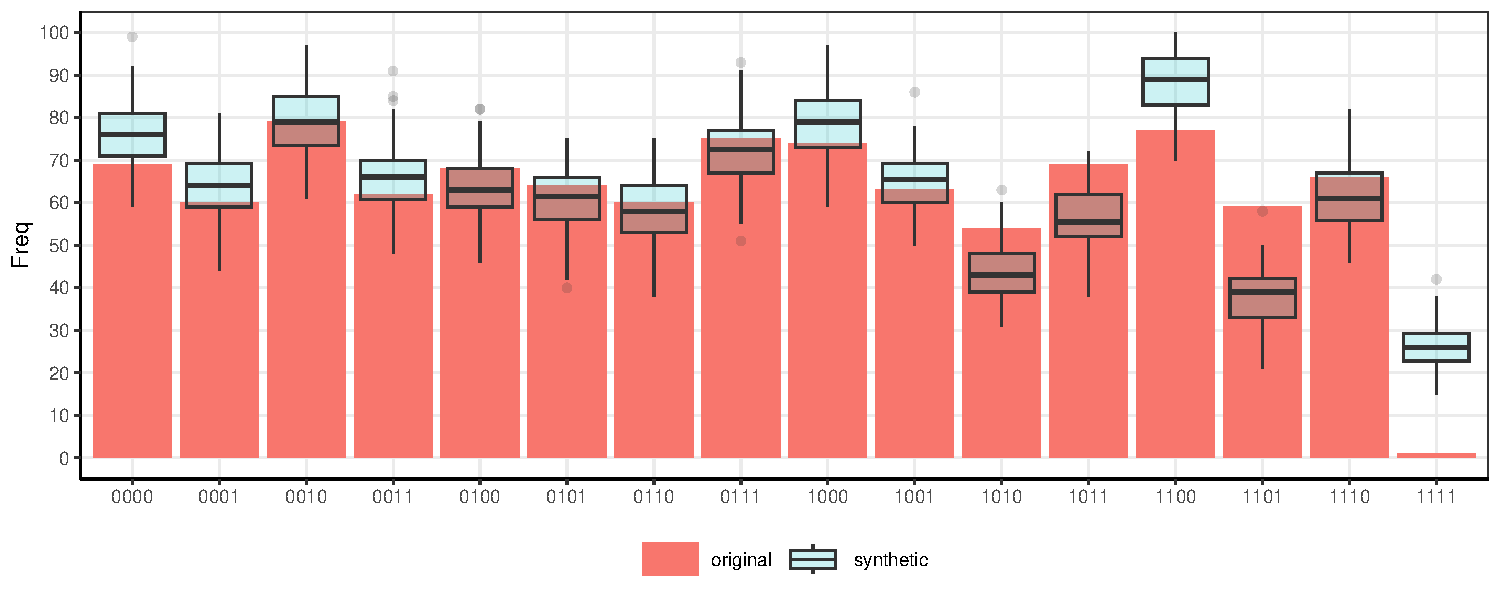
\includegraphics{../../graphs/graph_categorical_compare_histogram_100.pdf}}
    \label{fig:graph_categorical_compare_histogram_100}
\end{figure}
}

%%%%%%%%%%%%%%%%%%%%%%%%%%%%%%%%%%%%%%%%
%%%%%%%%%%%%%%%%%%%%%%%%%%%%%%%%%%%%%%%%
\section{Measuring utility and privacy}\label{sec:measuring}
%%%%%%%%%%%%%%%%%%%%%%%%%%%%%%%%%%%%%%%%
%%%%%%%%%%%%%%%%%%%%%%%%%%%%%%%%%%%%%%%%
\frame{\frametitle{Comparing utility measures}
\begin{figure}
    \caption{Utility measures close to 0, i.e. high utility}
    \resizebox{\textwidth}{!}{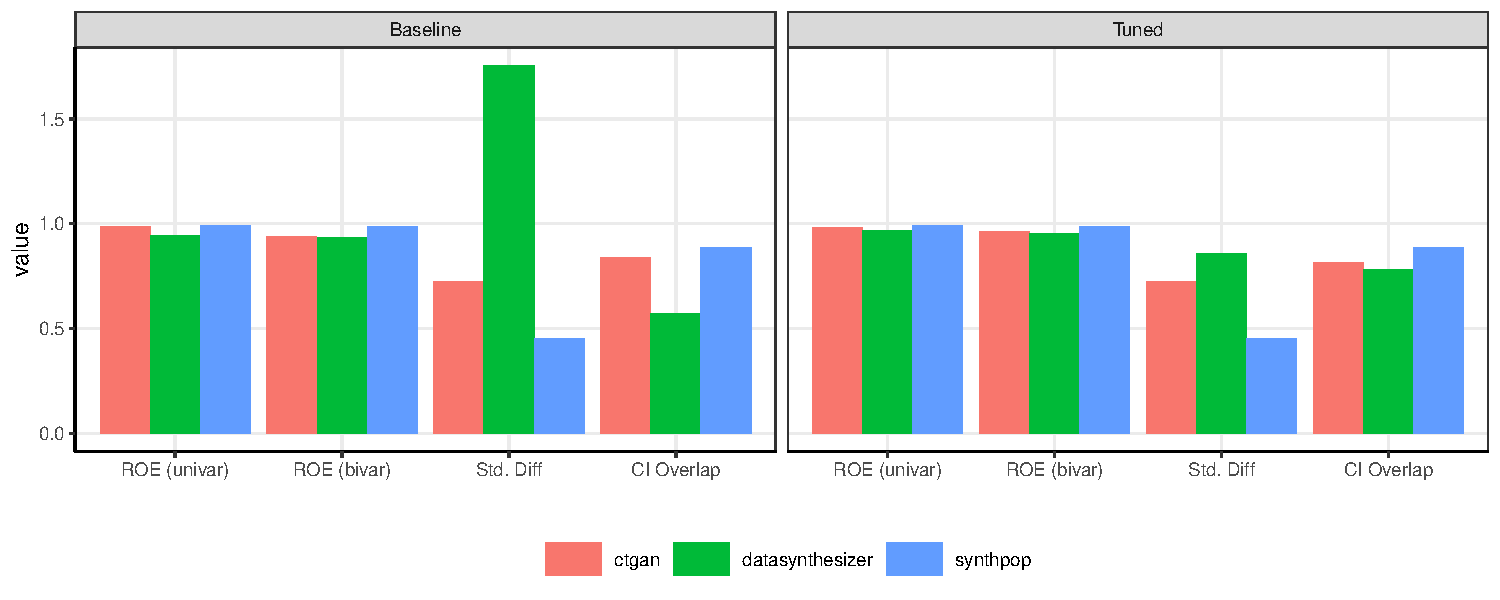
\includegraphics{../../graphs/graph_compare_utility.pdf}}
    \label{fig:graph_compare_utility}
\end{figure}
}

\frame{\frametitle{Comparing privacy measures}
all privacy measures close to 0, i.e. low privacy risk
}

%%%%%%%%%%%%%%%%%%%%%%%%%%%%%%%%%%%%%%%%
%%%%%%%%%%%%%%%%%%%%%%%%%%%%%%%%%%%%%%%%
\section{How do we explain this?}\label{sec:explain}
%%%%%%%%%%%%%%%%%%%%%%%%%%%%%%%%%%%%%%%%
%%%%%%%%%%%%%%%%%%%%%%%%%%%%%%%%%%%%%%%%
\frame{\frametitle{How do we explain this?}
\begin{figure}
    \caption{}
    \resizebox{\textwidth}{!}{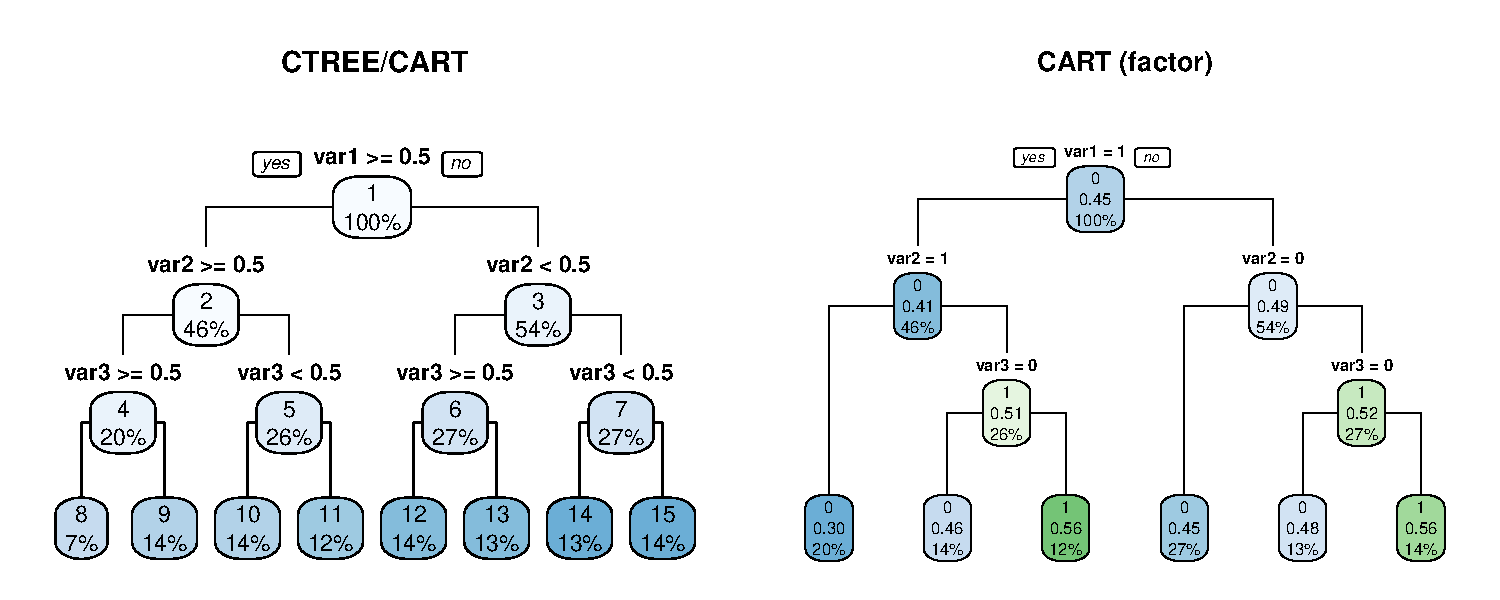
\includegraphics{../../graphs/graph_tree_combined.pdf}}
    \label{fig:graph_tree_combined}
\end{figure}
}

\frame{\frametitle{Histogram with differential privacy x 100 simulations}
\begin{figure}
    \caption{}
    \resizebox{\textwidth}{!}{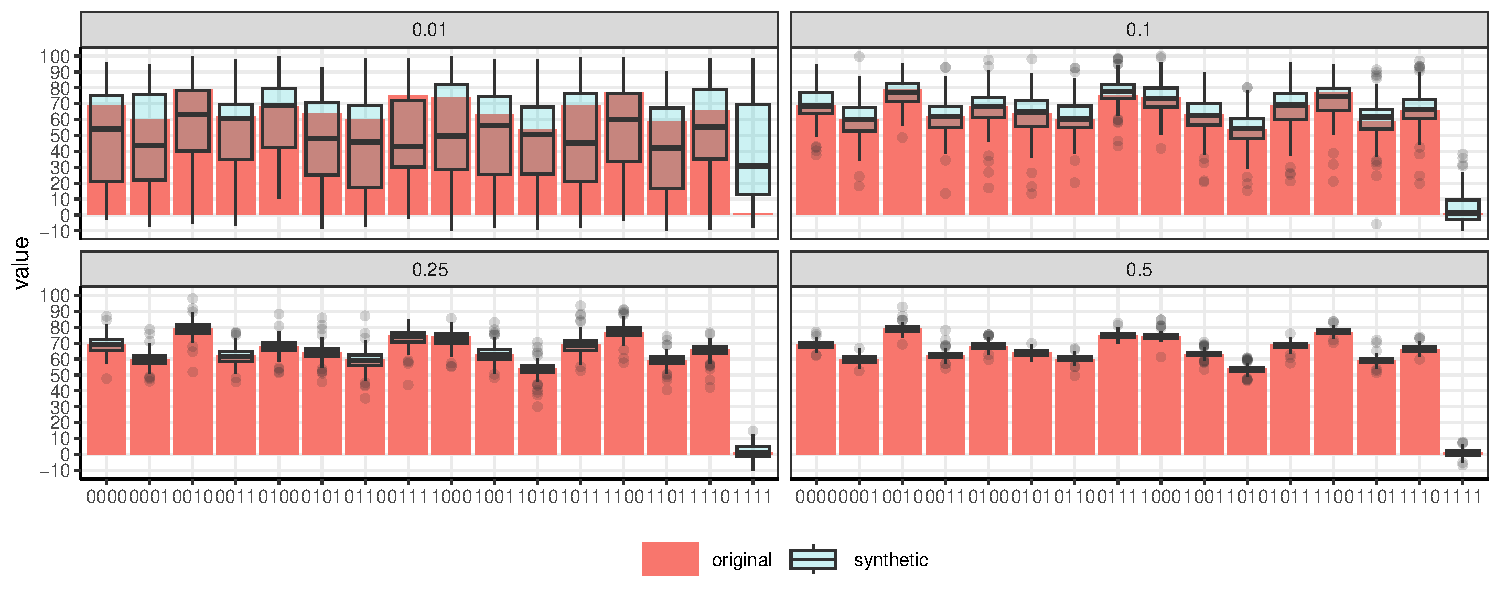
\includegraphics{../../graphs/graph_dp_compare_histogram_100.pdf}}
    \label{fig:graph_dp_compare_histogram_100}
\end{figure}
}

\frame{\frametitle{Histogram with DP (datasynthesizer) x 100 simulations}
\begin{figure}
    \caption{}
    \resizebox{\textwidth}{!}{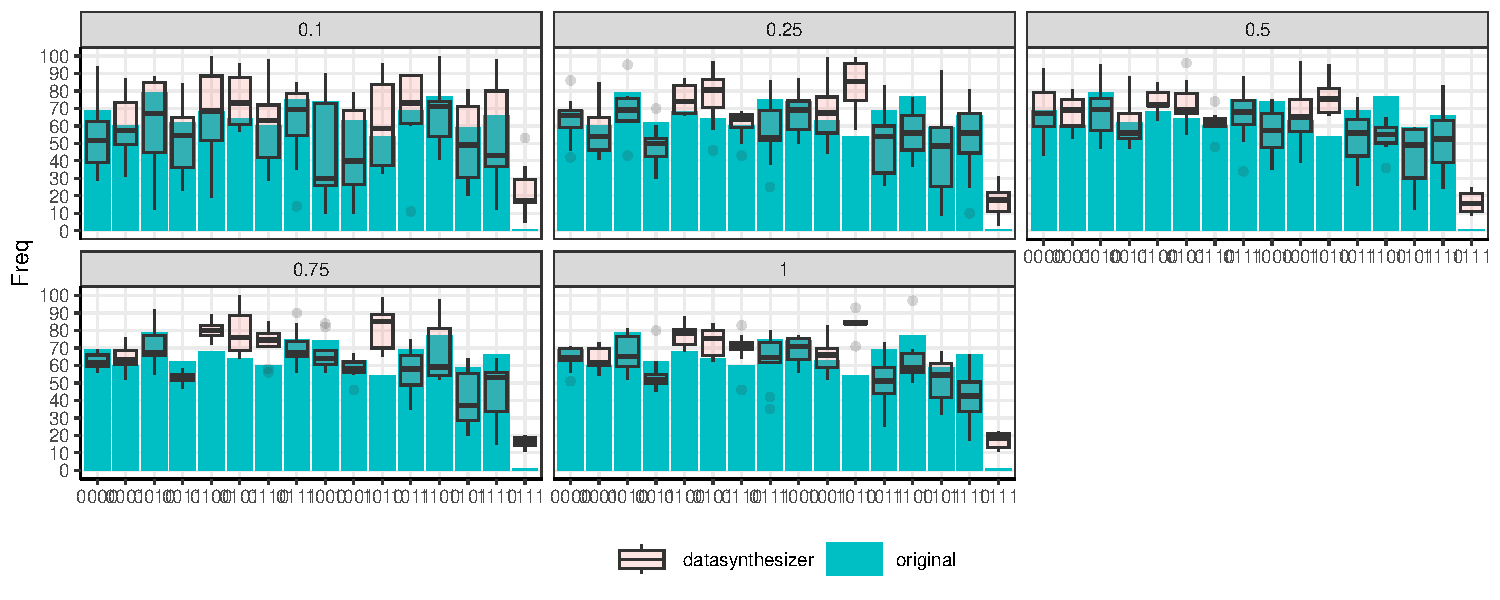
\includegraphics{../../graphs/graph_dp_datasynthesizer_compare_histogram_100.pdf}}
    \label{fig:graph_dp_datasynthesizer_compare_histogram_100}
\end{figure}
}



\end{spacing}
\end{document}

